\documentclass[11pt,DIV=15]{scrreprt}
\usepackage{ucs}
\usepackage[utf8x]{inputenc}
\usepackage[T1]{fontenc}
\usepackage[ngerman]{babel}
\usepackage[ilines,footsepline]{scrpage2}
\usepackage{listings}
\usepackage[hyphens]{url}
\usepackage[colorlinks=false, pdfborder={0 0 0}]{hyperref}
\usepackage{graphicx}
\urlstyle{tt}
\lstset {breaklines=true}
\graphicspath{ {./images/png/} }


\title{Windows Service Information}
\author{Jan Graefe}




\begin{document}
\maketitle
\tableofcontents
\chapter{Einleitung}
WindowsServiceInformation ist ein Framework zum Sammeln von Informationen über auf einem System installierte Dienste. \\

Dieses Dokument beschreibt zum einen das Tool WSI.EXE, zum anderen das dahinter liegende WindowsServiceInformation Framework.\\

Mit WSI.EXE steht ein anwendungsbereite Implementation des Frameworks zu Verfügung.\\

Die Kenntnis des Frameworks ermöglicht die Erstellung von eigenen Erweiterungen (Extensions) für WSI.EXE.\\

Weiterhin kann mit diesen Kenntnissen auch die Implementation einer eigenen Anwendung erfolgen.
\chapter{WindowsServiceInformation Konsolenanwendung WSI.EXE}
\section{Funktionsweise}
WindowsServiceInformation (WSI.EXE) ist ein Kommandozeilen-Tool um Informationen über Windows Dienste auf einem bestimmten System zu einem bestimmten Zeitpunkt zu sammeln und zu Dokumentationszwecken auszugeben. \\
Das Programm kann wie folgt aufgerufen werden:
\begin{lstlisting}
$> wsi.exe -s [Servicefilter] -o [Ausgabepfad] --type [Ausgabetyp]
\end{lstlisting}
\begin{itemize}
 \item[-s] Optionaler Parameter zur Angabe eines Filters. Es werden nur Dienste berücksichtigt, die ganz oder zum Teil diesem Filter entsprechen.
 \item[-o] Opitonaler Parameter. Gibt den Ausgabenpfad an, in dem die generierten Dokumentationsdateien abgelegt werden. Wird dieser Parameter nicht übergeben, so werden die Informationen nur auf dem Bildschirm angezeigt und keine Ausgabedateien erzeugt.
 \item[--type] Pflichtparameter. Gibt an, in welchem Format die Informationen ausgegeben werden sollen. Per Standard unterstützt WSI die Typen \emph{WIKI} und \emph{INI}.
\end{itemize}


\section{Basisinformationen}
Dazu zählen standardmässig die folgenden Kriterien:

\begin{itemize}
	\item Name des Dienstes
	\item Anzeigename des Dienstes in der Windows Dienstverwaltung
	\item Starttyp des Dienstes (automatisch, manuell, deaktiviert ...)
	\item Benutzer, unter dem der Dienst ausgeführt wird
	\item Aktueller Status des Dienstes (ausgeführt, gestoppt ...)
	\item Pfad zur ausführbaren Datei des Dienstes
	\item Version dieser Datei	
\end{itemize} 

\ Diese Informationen werden im gewünschten Format ausgegeben.

\section{Anreicherung mit zusätzlichen Informationen}

Die Basisinformationen können mit zusätzlichen Informationen erweitert werden. Diese \glqq Anreicherung\grqq{} mit Daten ist optional und wird nicht durch das Standardsetup unterstützt. Die zusätzlichen Daten unterscheiden sich von Dienst zu Dienst. Hierfür müssen Extensions eingebunden werden.  Die Extension muss die Dienste somit auf Basis der gewonnene Standardinformationen unterscheiden und die Daten auf geeignete Art und Weise hinzufügen.

\section{Verarbeitung von Konfigurationsdateien}
Dienste können unterschiedliche Konfigurationsdateien besitzen. Eine Extension kann dies berücksichtigen und die Basisinformationen des Dienstes mit dem Ablageort zu einer oder mehreren Konfigurationsdateien anreichern. WSI legt dann eine Kopie der Konfigurationsdatei unterhalb des Ausgabeverzeichnisses ab. Es wird dabei pro Dienst ein Unterverzeichnis mit dem jeweiligen Dienstnamen angelegt. Dieser Funktion ist nur mit dem Parameter \emph{--type WIKI} verfügbar!

\section{Verwendung von Erweiterungen (Extensions)}
Hervorgehend aus den vorherigen Kapiteln liegt die wahre Stärke von WSI in den Extensions. Ohne Extension liefert WSI nur die Basisinformationen. Soll eine Extension verwendet werden, so muss diese in der WSI.config hinterlegt werden. 

\begin{lstlisting}
    <applicationSettings>
        <WindowsServiceInformationConsole.Properties.Settings>
            <setting name="ExtensionDLL" serializeAs="String">
                <value>MyWsiExtension.dll</value>
            </setting>
        </WindowsServiceInformationConsole.Properties.Settings>
    </applicationSettings>
\end{lstlisting}

\chapter{WindowsServiceInformation Framework}

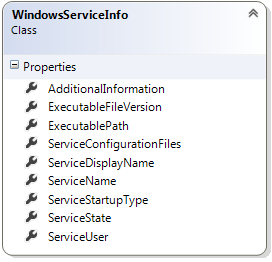
\includegraphics{Class_WindowsServiceInformation.png}

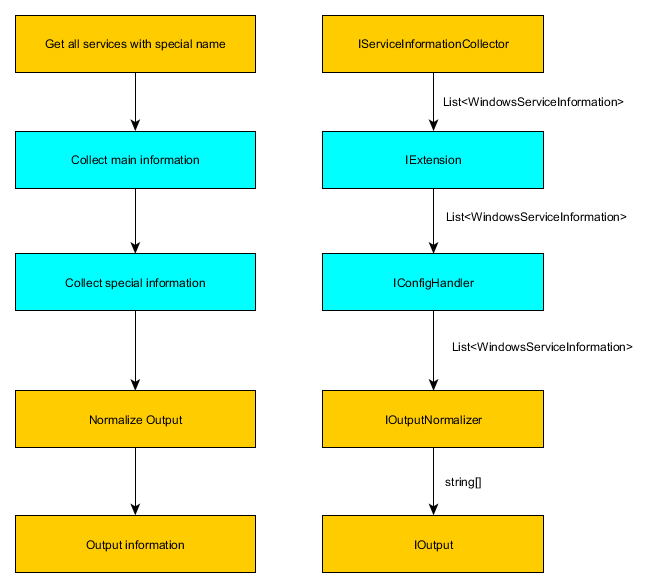
\includegraphics[scale=0.65]{WSI_Concepts_generic.png}


\begin{lstlisting}
namespace ch.jaxx.WindowsServiceInformation
{
    /// <summary>
    /// Class provides information about a windows service.
    /// </summary>
    public class WindowsServiceInfo
    {
        /// <summary>
        /// Service name as displayed in windows service manager.
        /// </summary>
        public string ServiceDisplayName { get; set; }
        /// <summary>
        /// Service name.
        /// </summary>
        public string ServiceName { get; set; }
        /// <summary>
        /// Running state of the service.
        /// </summary>
        public string ServiceState { get; set; }
        /// <summary>
        /// Service startup type (manual, automatic)
        /// </summary>
        public string ServiceStartupType { get; set; }
        /// <summary>
        /// Service user as set in service control manager
        /// </summary>
        public string ServiceUser { get; set; }
        /// <summary>
        /// Path to service executable.
        /// </summary>
        public string ExecutablePath { get; set; }
        /// <summary>
        /// A list of valid configuration files for this service instance
        /// </summary>
        public List<string> ServiceConfigurationFiles { get; set; }
        /// <summary>
        /// FileVersion of the service executable.
        /// </summary>
        public string ExecutableFileVersion { get; set; }
        /// <summary>
        /// An unmanaged string list with additional information.
        /// </summary>
        public List<WindowsServiceExtraInfo> AdditionalInformation { get; set; }
       
    }

\end{lstlisting}
\end{document}